% Status: Zweitprüfung

\section{Verwendete Technologien}
Im folgenden Abschnitt werden die Technologien beschrieben, die durch das FreeDesign-Projekt genutzt werden. 

\subsection{Representation State Transfer (REST)}
Der \emph{Representation State Transfer}-Architekturstil beschreibt die Kommunikation zwischen verteilten Softwaresystemen auf der Basis des HTTP-Protokolls und mit dem Ziel der hohen Unabhängigkeit der Einzelkomponenten des Systems. \autocite[vgl.][105-106]{Fielding2000}.

Zur Kommunikation und dem Dateienaustausch mit den Webservern der Portale, in denen der FreeDesign-Editor integriert ist, wird eine Vielzahl von REST-Webservices genutzt. 
Beispiele für Daten die ausgetauscht werden, sind Produktinformationen, Nutzerdaten oder Datenstrukturen für Designs, die in Datenbanken abgelegt sind.
Die Webservices werden durch ein eigenes Team innerhalb der IT-Abteilung betreut.  

\subsection{TypeScript}
Für die Implementation des FreeDesign-Editors wird die von Microsoft entwickelte Programmiersprache TypeScript\footnote{Weiterführende Informationen zu \emph{TypeScript}: \url{https://www.typescriptlang.org}} eingesetzt. TypeScript erweitert Javascript um statische Typinformationen und um das Konzept der objektorientierten Programmierung. Dies erhöht die Lesbarkeit des Quelltextes und dient der Vermeidung von Fehlern \autocite[vgl.][S. 111]{Zeigermann2014}. 

Der TypeScript Quelltext wird für die Ausführung im Browser in Javascript übersetzt. Damit ist TypeScript für große Projekte mit mehreren Teammitgliedern, wie dem FreeDesign-Editor, geeigneter als die Implementation in purem Javascript.

\subsection{ReactJS}
Für die Entwicklung einer SPA empfiehlt sich der Einsatz eines Frameworks oder einer Library, welches diesen Ansatz unterstützt. Im FreeDesign-Projekt wird die \emph{ReactJS}\footnote{Weiterführende Informationen zu \emph{ReactJS}: \url{https://reactjs.org}}-Library, welche von Facebook entwickelt wird, eingesetzt.
Basierend auf der Dokumentation von Facebook (\cite{Facebook:React}) kann die Funktionalität der React-Library wie folgt zusammengefasst werden.
Eine mit React erstellte Applikation setzt sich aus einer Vielzahl von React-Komponenten zusammen. Jede React-Komponente besitzt Eigenschaften, die bei dem Instanziieren einer Komponente mit Werten versehen werden, sowie einem internen Statusobjekt, welches innerhalb der Komponente verändert werden kann. 
Das zentrale Element einer React-Komponente ist das Erzeugen eines HTML-Knoten zur Darstellung der Komponente innerhalb der Applikation. Die Erzeugung des HTML-Knotens basiert auf den Kombination-Eigenschaften und dem Statusobjekt.
Verändern sich die Eigenschaften oder das Statusobjekt, wird dies von der React-Komponente registriert und das Erzeugen des HTML-Knoten wird erneut ausgeführt. Innerhalb des HTML-Knotens, können weitere React-Komponenten instanziiert und somit in die HTML-Struktur integriert werden.

\subsection{Redux}
Eine Herausforderung für jede SPA ist die Verwaltung applikationsübergreifender Daten sowie das Aktualisieren der Applikation bei Veränderung der Daten.
Einen flexiblen Ansatz bietet die Javascript-Bibliothek \emph{Redux}\footnote{Weiterführende Informationen zu \emph{Redux}: \url{https://redux.js.org}}, welche für die Verwaltung des Status einer SPA entwickelt wurde \autocite[vgl.]{Redux:Introduction}. 
Durch die Erweiterung \emph{React-Redux} funktioniert Redux besonders gut in Verbindung mit React.
Das Redux-Konzept in Verbindung mit React kann, basierend auf der Projekt-Dokumentation (\cite{ReactRedux:QuickStart}) wie folgt umrissen werden. Bei Start der React-Anwendung wird ein zentrales Javascript-Objekt erzeugt, welches sämtliche Statusinformationen der Anwendung enthält. Dieser sogenannte \emph{Store} wird ausschlich durch Redux verwaltet. Die React-Redux-Bibliothek stellt ein \emph{Provider}-Objekt zur Verfügung, welches Redux, das Store-Objekt und die React-Anwendung miteinander verbindet. Von der selben Bibliothek wird eine \emph{connect}-Funktion bereitgestellt, mit deren Hilfe Properties einer React-Komponente an Daten des Store-Objektes gebunden werden können. Ist es notwendig Informationen im Store zu ändern, geschieht dies durch den Aufruf einer \emph{Action}, was an jeder Stelle der Applikation geschehen kann. Aufgerufene Actions werden von sogenannten Reducern verarbeitet und erzeugt, basierend auf der Action ein neues Store-Objekt, welches durch Redux aktualisiert wird. Dieser so entstehende Zyklus wird in Abbildung \ref{figure:ReduxCycle} dargestellt.
\begin{figure}[H]
\centering
\efbox{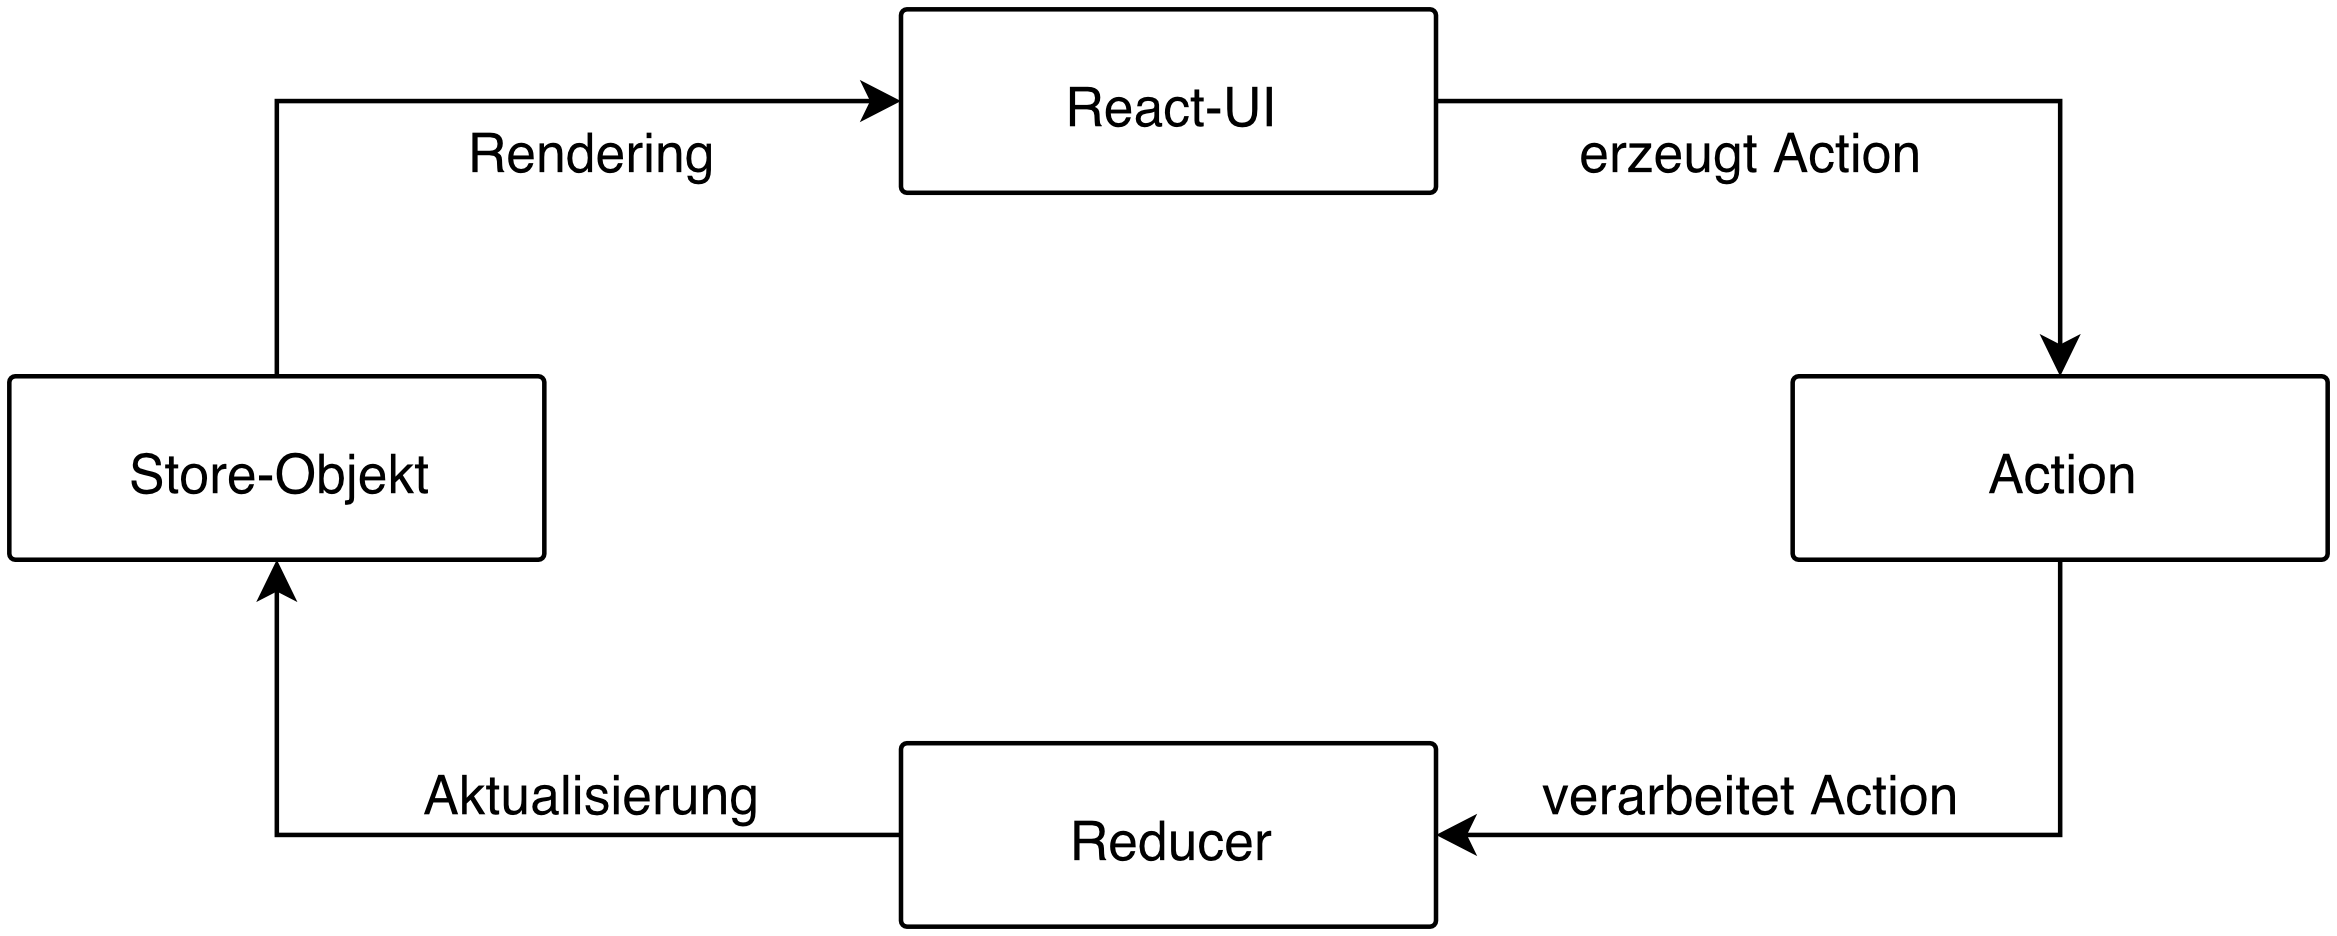
\includegraphics[width=.98\linewidth]{diagrams/ReduxCycle.png}}
\caption[Redux-Zyklus]{der Redux-Zyklus}
\label{figure:ReduxCycle}
\end{figure}
Redux gibt somit einen Kreislauf der Verarbeitung applilaktionsübergreifender Daten vor und bewirkt somit, dass die Darstellung der React-Applikation stets auf dem Store basiert.


\subsection{Jest und Enzyme}
Zum Erstellen von Unit-Tests wird das Testing-Framework Jest \footnote{Das Testing-Framework \emph{Jest} ist unter Url \url{https://jestjs.io} dokumentiert.} eingesetzt, da es ebenfalls durch Facebook entwickelt wird und somit höchstmögliche Kompatibilität mit den React-Komponenten bietet. Weiterhin bietet das Framework als Besonderheit die Erstellung von \emph{Snapshot-Tests}, mit deren Hilfe es sehr einfach ist, die korrekte Struktur von großen Objekten, wie das Rendering von React-Komponenten, sicherzustellen \autocite[vgl.][]{Facebook:JestIntroduction}.
Die Tests werden mit dem Kommandozeilenbefehl \emph{jest} ausgeführt.
Beim Ausführen der Tests analysiert Jest das Projekt,  erfasst automatisch Test-Dokumente und führt diese aus. 
Die Erfassung der Test-Dokumente kann jedoch auch eingeschränkt werden, indem bei der Ausführung der Tests ein Teil des Dokumentennamen übergeben wird. Dies beschleunigt den Aufruf einzelner Tests. 
Ergänzt wird der Einsatz des Jest-Frameworks durch die Nutzung der Funktionsbibliothek \emph{Enzyme}\footnote{\emph{Enzyme} ist unter \url{https://enzymejs.github.io/enzyme/} dokumentiert.}. Enzyme wurde speziell für das Testen von React-Komponenten entwickelt und bietet Funktionalitäten, die das Testen von React-Komponenten erleichtern \autocite[vgl.][]{Enzyme:Introduction}.

\subsection{Das SVG-Format}
Das \emph{Scalable Vector Graphics}-Format (SVG) ist eine XML-basierte Markup-Sprache, welche eine Vektorgrafik beschreibt. SVG-Grafiken können als *.svg-Dateien gespeichert und innerhalb von HTML-Quelltext platziert werden \autocite[vgl.][]{W3C:AboutSVG}. 

Innerhalb des FreeDesign-Editors wird das SVG-Format für die Produkt- und Designdarstellung sowie für die Darstellung von Bearbeitungswerkzeugen eingesetzt. 

\subsection{Git}
\label{chap:git}
Zur zentralen Quelltextverwaltung nutzt Unitedprint das Versionsverwaltungssystem \emph{Git}, welches Dateiänderungen protokolliert und diese Versionen zuweist. Dadurch ist es möglich jede Änderungen im nachhinein nachzuvollziehen, mit einem vorhergehenden Zustand zu vergleichen und bei Bedarf rückgängig zu machen \autocite[vgl.][]{Git:About}.

Weiterhin bietet Git die Möglichkeit verschiedene Zustände eines Projektes in sogenannten \emph{Branches} zu verwalten, wobei jedes Git-Projekt einen eigenen Haupt-Branch besitzt. Um diesen während der 
Entwicklung nicht zu beeinflussen, können Änderung in eigenen Branches entwickelt werden und nach Abschluss der Entwicklungsarbeit mit dem Haupt-Branch zusammengeführt werden \autocite[vgl.][]{Git:Branching}. 

Git bietet eine Vielzahl weiterer Funktionalitäten, um mit Branches zu arbeiten, deren Beschreibung jedoch für das Verständnis der vorliegenden Diplomarbeit nicht notwendig ist. 

Für das zentrale Management von Git-Projekten setzt Unitedprint die Software Bitbucket ein, welches von einem IT-internen Operations-Team verwaltet wird. Über Bitbucket können Entwickler die Integration eines Branches in einen anderen Branch beantragen, was als Pull-Request bezeichnet wird. Pull-Requests können von anderen Entwicklern begutachtet werden und Änderungen am Projektinhalt kommentiert werden. Weiterhin bietet Bitbucket die Funktionalität sogenannter Pipelines, mit deren Hilfe automatisiert Integrationsschritte ausgeführt werden können \autocite[vgl.][]{Bitbucket:Product}.

Das FreeDesign-Projekt wird in einem eigenem Git-Projekt verwaltet.
